

\hspace{5mm} Modern vehicles rely on a distributed electronic architecture composed of multiple interconnected control systems that continuously monitor and manage vehicle operation. At the core of this architecture are ECUs, which process data from numerous sensors and coordinate the operation of vehicle subsystems to ensure optimal performance, efficiency, safety, and compliance with regulatory requirements. ECUs are responsible for controlling engine sensors and actuators, as well as providing various vehicle operating parameters such as engine speed (RPM), pressures, temperatures, air-fuel mixture, and other relevant indicators \cite{jg}.



\section{Vehicular Communication Networks}

\subsection{Electronic Control Unit}

It functions as a small embedded computer, acquiring information from sensors, processing this data in real time, and sending commands to actuators. Depending on its purpose, an ECU may control the engine, transmission, ABS braking system, stability control, power steering, airbags, and many other systems found in modern automobiles \cite{jg}.

The development of ECUs became increasingly relevant during the 1970s and 1980s, driven by the need to improve engine efficiency and reduce pollutant emissions. 

Before the development of ECU, automotive systems were mostly mechanical. As vehicles became more a more complex and had more stict regulations, there was a need for more precise electronic solutions, leading to the creation of the first ECUs


\subsection{Controller Area Network}


The \ac{CAN} Network is a vehicle message-based communication protocol design to allow an ECU to communicate to other devices without the need for a central computer and to enable a fast and reliable exchange of information between electronic modules \cite{iso11898}. 

This protocol was developed by Robert Bosch GmbH in the 1980s as a response to the increasing complex vehicular systems of the time. Over time, the CAN protocol became the standard due to it's simplicity and ability to operate in electrically noisy environment.

\begin{figure}[H]
  	\centering   
    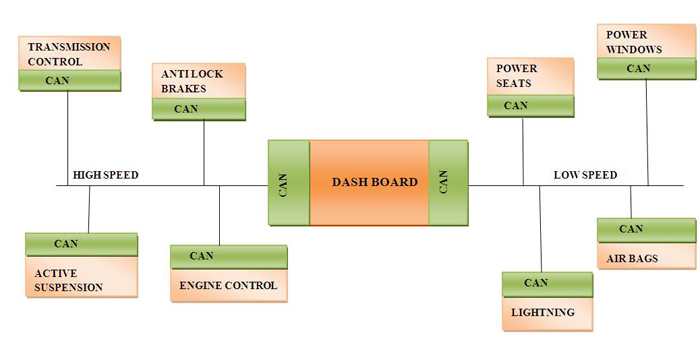
\includegraphics[width=0.8\linewidth]{imagens/Can_protocol.png}
    \caption{CAN Application Example \cite{canprotocol}}
    \label{fig:prj_arch}
\end{figure}

CAN protocol is a message-based protocol. This means the data of a vehicule is transmitted in messages identified by a unique ID and available for every electronic module to read, instead of being sent to specific devices. Any ECU on the network can broadcast messages, and any other ECU can choose to listen to the messages relevant to it.

These messages, known as frame, follow a specific format as to ensure consistency:
\begin{itemize}
    \item ID - Unique message identifier
    \item DLC (Data Length Code) - Specifies the data length in bytes
    \item Data Field - Contain the information payload 
    \item CRC (Cyclic Redundancy Check) - Used for error and data integrity verification
    \item ACK Slot - Confirms reception of at least one node
    \item EOF (End of Frame) - Signals the end of the message
\end{itemize}

\begin{figure}[H]
  	\centering   
    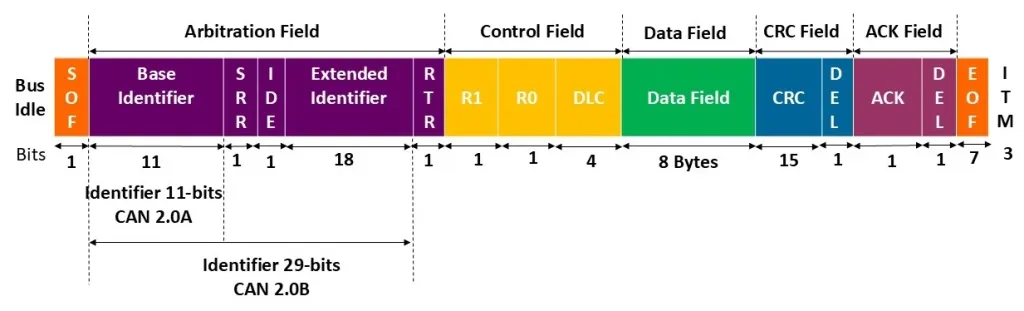
\includegraphics[width=1\linewidth]{imagens/CAN-Protocol-Extended-Frame-Format.png}
    \caption{CAN Standard Data Frame \cite{canframe}}
    \label{fig:prj_arch}
\end{figure}


\subsection{Controller Area Network Data Base}

CAN databases, commonly represented as DBC files, play a fundamental role in the interpretation and use of CAN bus data in modern automotive and embedded systems. A CAN database defines the structure and semantics of CAN messages, enabling the translation of raw binary frames into meaningful physical signals.
A CAN frame, by itself, only contains an identifier and a sequence of data bytes. Without additional context, this data is not directly interpretable. CAN databases address this limitation by providing a structured description of each message, including its identifier, length, and the layout of individual signals within the payload. Each signal is defined through parameters such as bit position, bit length, scaling factor, offset, and engineering units. This makes it possible to convert raw byte streams into values such as engine speed in revolutions per minute, throttle position, or air fuel ratio \cite{vectorcandb}. 
One of the primary use cases of CAN databases is real-time data decoding. In systems such as ECU monitoring platforms or vehicle telemetry applications, incoming CAN frames are matched against database definitions and decoded into structured data. This enables the development of dashboards, logging systems, and diagnostic tools that present meaningful information to the user. In the context of the proposed solution, the DBC file is used to decode messages from a rusefi ECU, translating low level CAN frames into a normalized vehicle state.
Another relevant application is data logging and offline analysis. CAN databases allow raw CAN traffic to be recorded while preserving the ability to decode it at a later stage. This is particularly useful for debugging, performance evaluation, and research activities. Since decoding logic is defined externally in the database, previously recorded data can be reinterpreted using updated signal definitions without requiring any modification to the stored dataset.
CAN databases are also widely used in simulation and testing environments. By defining message structures and signal properties, DBC files allow synthetic CAN traffic to be generated in a controlled manner. This capability is important in hardware in the loop and software validation scenarios, where realistic communication patterns are required without relying on physical ECUs.
Additionally, DBC files contribute to standardization and interoperability across different tools and systems. Multiple applications such as CAN analyzers, embedded controllers, and data acquisition platforms can use the same database to ensure consistent interpretation of CAN messages. This reduces ambiguity and simplifies integration in complex systems involving multiple components and suppliers \cite{pfeiffer}.

\subsection{Why CAN is the Preferred Method for Intra-Vehicular Communication}

Controller Area Network (CAN) is widely adopted in intra-vehicular communication due to its deterministic behavior, fault tolerance, and efficient bus architecture. It is specifically designed for distributed embedded systems where multiple ECUs must exchange time-critical information over a shared medium \cite{bosch}.

CAN employs a multi-master, message-oriented communication model over a differential two-wire bus, which increases noise immunity in electrically harsh automotive environments. Reliability is ensured through multiple built-in mechanisms, including CRC, bit stuffing, frame validation, and automatic retransmission upon error detection. Fault confinement is also supported, allowing malfunctioning nodes to be isolated from the network.

A key feature of CAN is its non-destructive bitwise arbitration mechanism, which guarantees deterministic access to the bus. Message priority is encoded in the identifier field, where lower numerical values correspond to higher priority. During arbitration, nodes transmit simultaneously and monitor the bus, withdrawing transmission if a dominant bit is overwritten by a recessive bit. This ensures that the highest priority message is transmitted without collision or delay.

In terms of efficiency, CAN minimizes wiring complexity by using a shared bus topology, reducing both system cost and physical weight. It supports data rates up to 1 Mbps in Classical CAN, which is sufficient for most control applications. The protocol also allows both 11-bit and 29-bit identifiers, enabling flexible message addressing schemes, as shown in Figure 2.2.

\subsection{Standalone ECU}

Standalone ECUs are aftermarket electronic control systems designed to fully replace the original equipment manufacturer (OEM) ECU. Their primary purpose is to provide greater flexibility, configurability, and control over engine operation, particularly in high-performance and motorsport applications.

Unlike OEM ECUs, which are typically optimized for emissions, reliability, and mass production constraints, standalone ECUs allow direct access to key engine parameters such as fuel injection, ignition timing, boost control, and sensor calibration. This enables precise tuning of engine behaviour according to specific requirements, such as performance optimization, component modifications, or experimental configurations.

The motivation for using standalone ECUs arises from the need for adaptability and transparency. In applications such as Formula Student, where vehicles are custom-built and continuously refined, engineers require full control over the engine management strategy. Standalone ECUs provide this capability by supporting user-defined maps, real-time parameter adjustment, and integration with external systems through communication protocols such as CAN.

\subsection{Speeduino/RusEFI ECUs}

Speeduino and RusEFI are open-source standalone ECU platforms designed to provide flexible and low-cost engine management solutions. Both systems aim to replicate and extend the functionality of commercial standalone ECUs, while maintaining full transparency and user control over hardware and software \cite{rusefi_website}.

Speeduino is based on Arduino-compatible hardware and focuses on simplicity and accessibility. It provides core engine control features such as fuel injection, ignition timing, and sensor processing, making it a popular choice for educational projects and low-budget motorsport applications. Its architecture allows easy integration with existing tools such as TunerStudio, enabling real-time tuning and data logging.

RusEFI, on the other hand, targets more advanced use cases with a higher level of performance and configurability. It typically runs on more powerful microcontrollers and offers extended features, including native CAN support, higher processing capabilities, and more precise control strategies. This makes it suitable for more demanding applications, such as competitive motorsport or complex engine setups \cite{rusefi_github}.

The main motivation behind both platforms is to provide open, customizable alternatives to proprietary ECUs. They allow users to modify control algorithms, extend communication interfaces, and integrate telemetry systems, such as the one proposed in this work. As a result, they are particularly well suited for environments like Formula Student, where flexibility, experimentation, and cost constraints are critical factors.

\section{Embedded System's Development Platforms}

\subsection{Raspberry Pi Ecosystem}

For the controller of our project, we decide to utilize a Raspberry Pi Zero 2W \cite{raspizero2w}. This decision was made due to several reasons:
\begin{itemize}
    \item \textbf{Full Linux Computer:} The controller will have to implement several different tasks at once such as:
    \begin{itemize}
        \item Real-time data aquisition from the ECU
        \item Data processing like filtering and parsing signals
        \item Database logging and managment
        \item UI rendering
        \item Real-time bluetooth data transfer
    \end{itemize}
    A Raspberry Pi system provides a good flexibility to develop our application while being able to build our application with the features above.
    \item\textbf{Fast processor and decent memory:}
    The Raspberry Pi Zero 2 W incorporates a quad-core 64-bit Arm Cortex-A53 CPU clocked at 1GHz, paired with 512MB of LPDDR2 SDRAM. This package provides the Raspberry Pi Zero 2 W with good performance for our application, and having multiple cores will help with our distributed system aproach.
    
    \item \textbf{Easy communication with hardware:} The Raspberry Pi provides a USB serial port with the possibility to use UART pins already built-in to the computer
    \item \textbf{Networking:} This computer provides a Bluetooth Low Energy (BLE) system which allows the transfer of the CAN signal information easily to a connected mobile device
\end{itemize}

With all this said, we choose the Raspberry Pi for its fast performance, and affordable price. Another deciding factor in the selection of this computer was the extensive community support, along with the large number of available open-source projects and software resources.


\subsection{Utilized Programming Languages}

Support for multiple programming languages was a key design consideration, allowing each component to leverage the strengths of the most appropriate language while mitigating its inherent limitations:
\begin{itemize}
    \item \textbf{Python:} Used for the controller application for a ECU data pipeline, controller logic and bluetooth integration due to it's simplicity for serial communication, data parsing and bluetooth features as well as extensive UI libraries;
    \item \textbf{SQLite:} Although Python is used for making requests to the database, said requests are in SQL using a SQLite variant due to being a light-weight alternative to variants like Postgres, for the simplicity of easy for there is no need for a database and instead SQLite stores information in a single file and has extremely fast writes which is perfect for storing the CAN dataframes obtained;
    \item \textbf{Kotlin:} Kotlin was chosen as the primary language for mobile application development due to its seamless integration with the Android platform, support for low-latency applications, comprehensive networking libraries, and the modern Jetpack Compose UI framework.
\end{itemize}


\section{Data Analysis Techniques in Motorsport}
\subsection{Statistical Analysis}

The data gathered by the ECU enables a wide range of analytical applications, including engine tuning, performance evaluation in track environments, and long-term data logging. These datasets provide valuable insights into the behaviour of the engine and associated subsystems under varying operating conditions.

The proposed system records a set of normalized vehicle parameters derived from CAN messages and stored periodically in the database. The currently logged parameters include:

\vspace{-0.2cm}
\begin{table}[H]
\centering
\begin{tabular}{|c|p{12cm}|}
\hline
\textbf{Parameter} & \textbf{Description} \\
\hline

RPM & Engine speed in revolutions per minute, primary indicator of engine operating speed.\\
\hline

SYNC & ECU/engine synchronization status, indicates whether the ECU has valid crankshaft and camshaft position information. \\
\hline

ENGINE & General engine operating status, useful for determining whether the engine is stopped, cranking, or running. \\
\hline

MAP & Intake manifold absolute pressure, one of the primary engine load measurements used for fuel calculations. \\
\hline

BARO & Ambient atmospheric pressure, used for altitude and weather compensation. \\
\hline

TPS & Throttle position, represents driver demand and throttle opening percentage. \\
\hline

IAT & Intake air temperature, affects air density and fueling calculations. \\
\hline

CLT & Engine coolant temperature, critical for warm-up enrichment and engine protection strategies. \\
\hline

AFR & Measured air-to-fuel ratio, key indicator of combustion mixture quality and engine tuning. \\
\hline

EGO & Fuel correction based on oxygen sensor feedback, represents closed-loop fueling adjustments applied by the ECU. \\
\hline

PW & Injector opening duration, directly relates to the amount of fuel delivered to the engine. \\
\hline

VE & Volumetric efficiency used in fuel calculations, represents how effectively the engine fills its cylinders with air. \\
\hline

ADV & Ignition timing advance, major factor of power output, efficiency, and knock resistance. \\
\hline

DWELL & Ignition coil charging time, determines the energy available for spark generation. \\
\hline

BAT & Electrical system voltage, important for injector operation, ignition performance, and system health monitoring. \\
\hline

BOOST & Target boost pressure, desired manifold pressure set by the ECU for forced-induction engines. \\
\hline

DUTY & Wastegate control duty cycle, indicates how aggressively the ECU is controlling boost pressure. \\
\hline

VSS & Vehicle speed, used for logging, speed-based strategies, and traction-related functions. \\
\hline

FAN & Cooling fan status, indicates whether the radiator cooling fan is active. \\
\hline

FP & Fuel pump status, shows whether the ECU has enabled the fuel pump output. \\
\hline

BOOSTCUT & Overboost protection status, indicates whether boost safety limits have been exceeded and protective intervention is active. \\
\hline

\end{tabular}
\caption{ECU Parameters Displayed by the Data Logger}
\label{tab:ecu_parameters}
\end{table}

\section{Bluetooth Integration}

\subsection{BLE Protocol}

Bluetooth Low Energy (BLE) is a short-range wireless protocol designed for
low-power, event-driven communication. Unlike Classic Bluetooth, BLE does not
maintain a continuous data stream. Instead, it organises data exchange around
the Generic Attribute Profile (GATT), where a peripheral advertises
its presence and exposes data, and a central scans for and connects
to it \cite{bleprimer}.

Within GATT, data is structured as services, containing one or more
characteristics. Each characteristic holds a value and a set of
permission flags. A \texttt{read} flag allows the central to request the
current value explicitly; a \texttt{notify} flag allows the peripheral to push
updates automatically once the central subscribes by writing to the
characteristic's Client Characteristic Configuration Descriptor (CCCD) \cite{bt54}.

\vspace{5mm}
\begin{figure}[H]
    \centering
    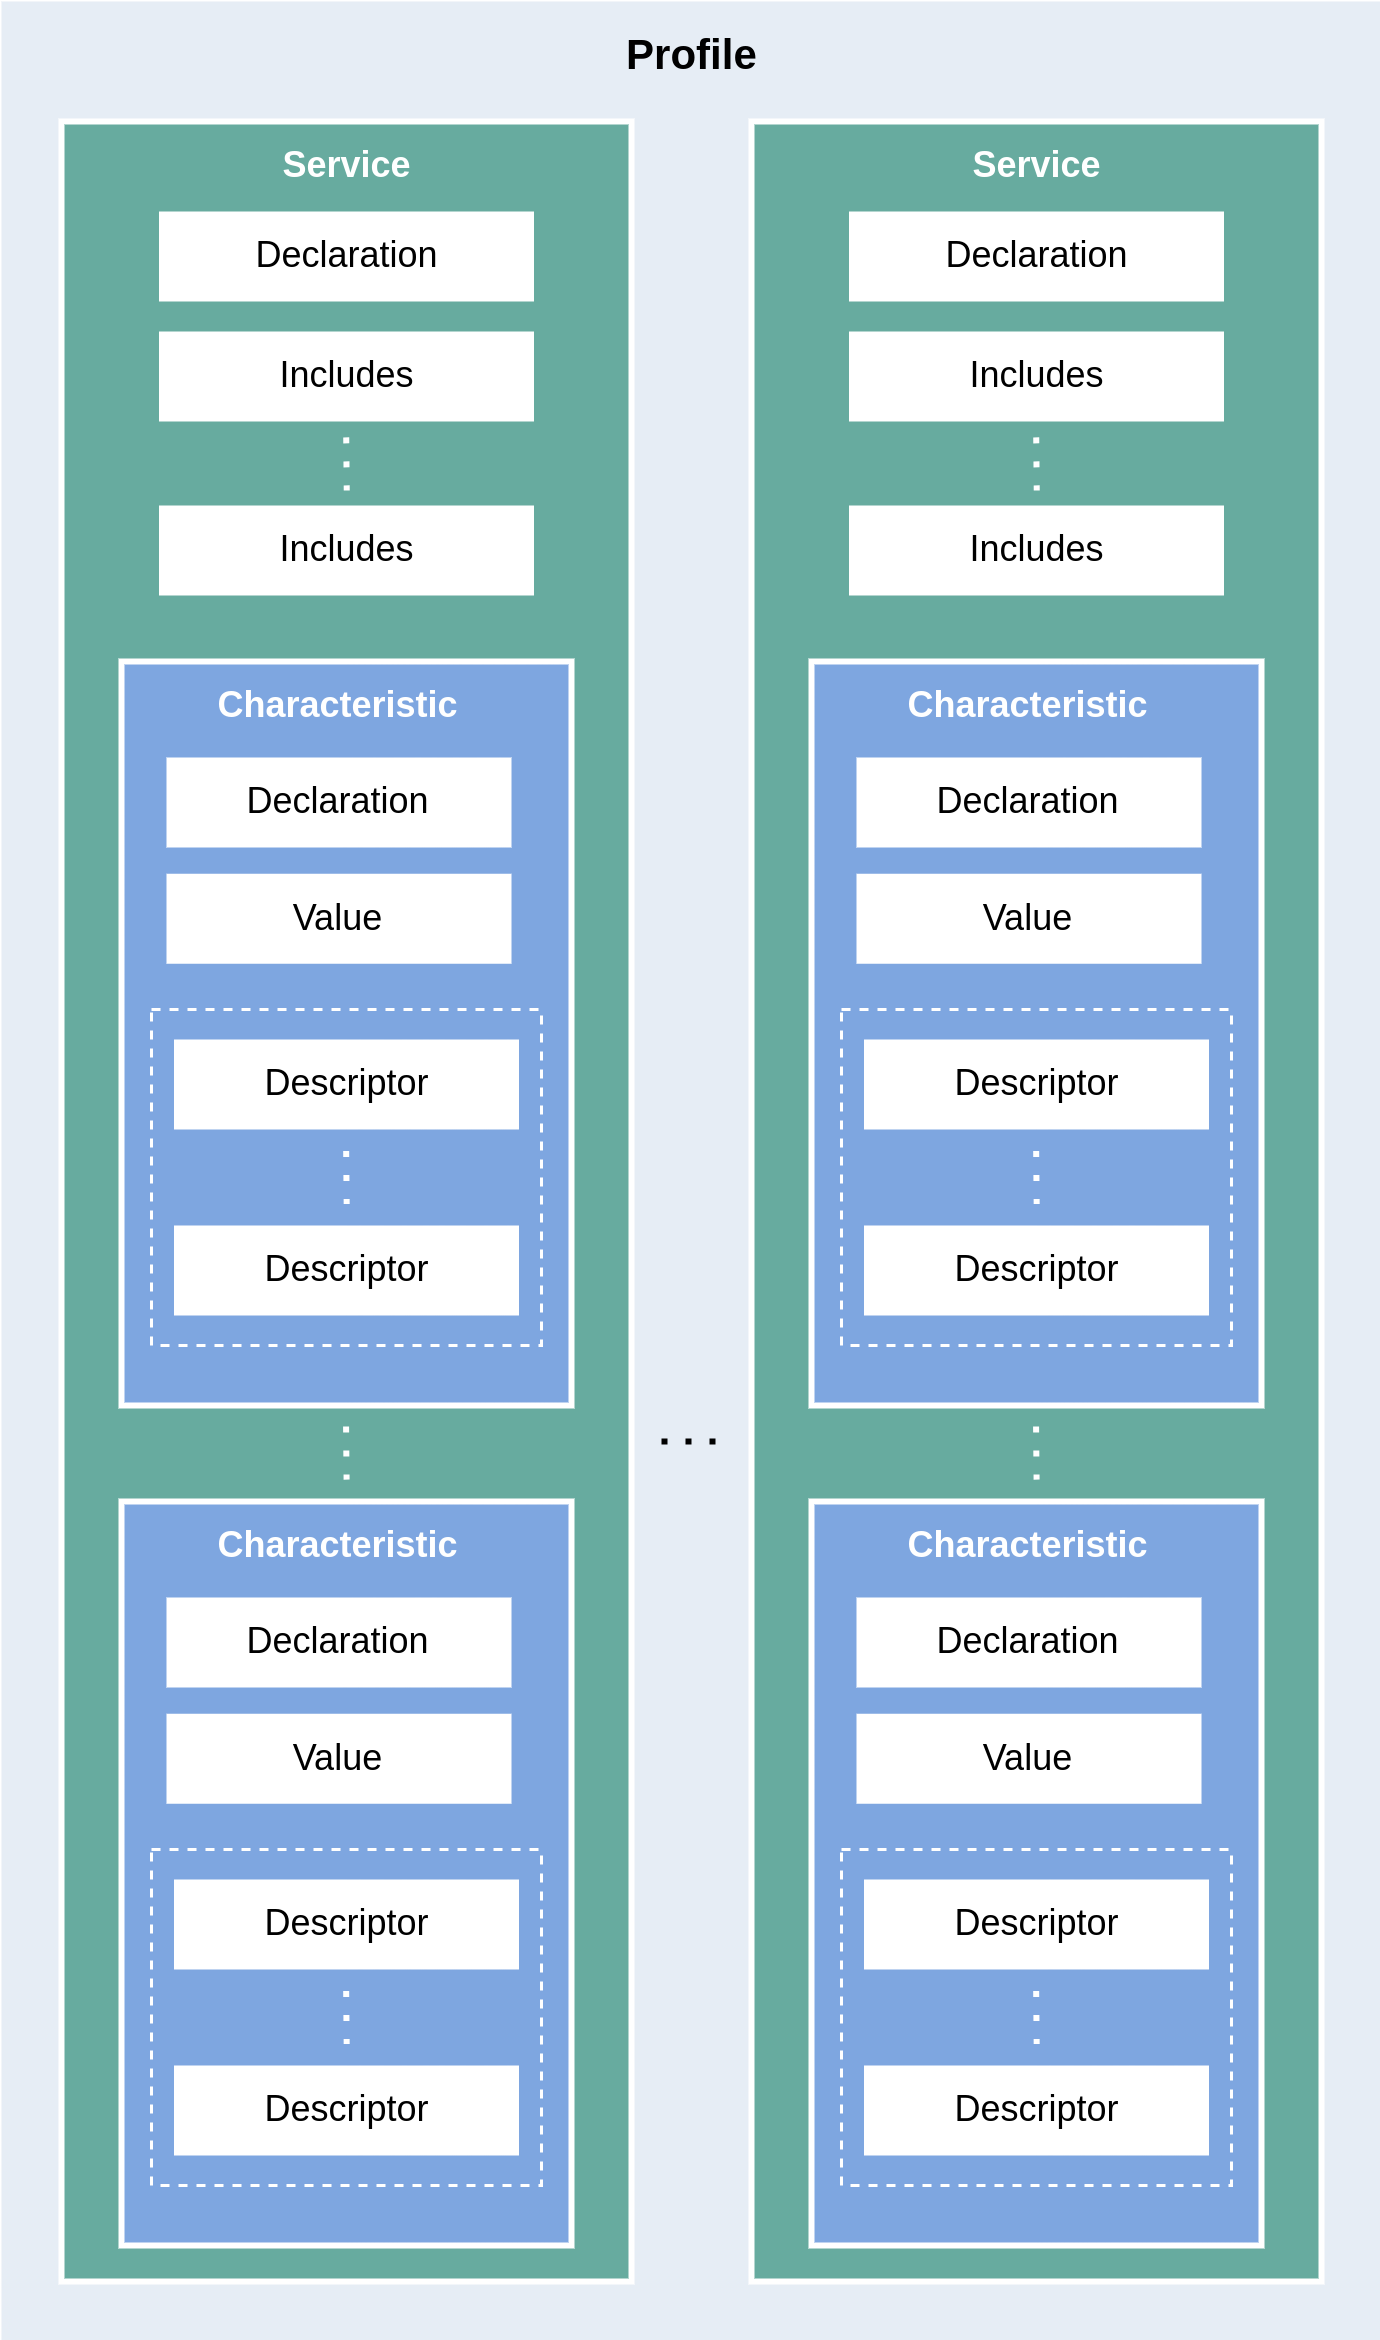
\includegraphics[width=0.5\linewidth]{imagens/ble-gatt-architecture.png}
    \caption{BLE GATT Hierarchical Architecture \cite{gatt}}
    \label{fig:placeholder}
\end{figure}
\vspace{5mm}

In our implementation, the \textit{bluezero} library is used to expose the
Raspberry Pi as a GATT peripheral over the Linux BlueZ stack via D-Bus.
A \texttt{Peripheral} object is configured with a service and its
characteristics, each assigned a Universally Unique Identifier (UUID), 
permission flags, and a callback. For \texttt{notify} characteristics, 
bluezero invokes the \texttt{notify\_callback} once on subscribe and once on 
unsubscribe, passing the live characteristic object. Periodic transmission is 
then driven by a GLib timer that calls \texttt{characteristic.set\_value()} at 
the desired interval, which BlueZ translates into a BLE notification delivered to 
the connected device. The server is started by calling \texttt{peripheral.publish()},
which hands execution to the GLib main loop indefinitely \cite{bluezero}.


\section{Project Synthesis and Differentiation}

In our analysis of the current alternatives to our project, we believe our implementation provides an alternative not seen in any other similar project for several reasons:

\begin{itemize}
    \item \textbf{Open-source:} Most alternatives are are not open-source, which make the modification or modular separation of each of it's components virtually impossible;
    \item \textbf{Modular Components:} Our project is separated in two different modules: Controller and Mobile App. Due to this, our project is flexible to the implementation of different alternatives as long as they are in accordance to the same communication protocol between modules;
    \item \textbf{Database integration:} From our research, every other alternative is a real-time monitoring. Ours gives the possibility of storing all the CAN dataframes in a database for posterior use, such as future simulations or statistical analysis;
    \item \textbf{Cross-plataform Accessibility:} Most options are purely limited to one plataform, be it a computer or a mobile device. Our implementation allows us to monitor the same data in different platforms at the same time, be it computer, mobile device or any other future device with a bluetooth connection;
    \item\textbf{Cheap and easy do aquire hardware:} Many other implementations utilize hard to source components, or may require a difficult setup.
\end{itemize}

Main close competitors to the proposed system:
 
\begin{itemize}
    \item Tuner Studio Dashboard(only dashboard) \cite{ts};
	\item uaDash(only dashboard)\cite{uadash};
	\item MegaLog viewer (only logger)\cite{mlviewer}.
\end{itemize}


